
\chapter{Desarrollo}
\label{cha:desarrollo}

\begin{FraseCelebre}
  \begin{Frase}
    Cada uno de nosotros debe trabajar para su propia mejora, y al mismo tiempo compartir una responsabilidad general para toda la humanidad.
  \end{Frase}
  \begin{Fuente}
    Marie Curie
  \end{Fuente}
\end{FraseCelebre}

\section{Introducción}
\label{sec:intro-desarrollo}

En el presente \gls{tfm} se ha desarrollado una estrategia de detección de objetos abandonados para ser aplicado en sistemas de videovigilancia. Como ya se comentó en la sección \ref{subsec:comparativa-detectores}, se utilizará como detector de objetos y personas \gls{yolov4} y como algoritmo de seguimiento \gls{deepsort}. A continuación, se describen las diferentes secciones que componen este capítulo.

Primero se evaluará YOLOv4 sobre Darknet, framework de código abierto escrito en C y \gls{cuda}, y se observará la precisión y velocidad que se obtiene en la detección de objetos y personas. Posteriormente se convertirá el modelo de \gls{yolov4} de Darknet a Tensorflow, framework de código abierto escrito en Python y C++ orientado al desarrollo de algoritmos inteligentes de Machine Learning. Utilizar \gls{yolov4} con Tensorflow facilitará la programación del algoritmo de detección de objetos abandonados con Python, ya que Darknet no es un framework de uso extendido y podría ser más difícil encontrar soluciones para los posibles errores. A continuación se reentrenará el modelo de la red \gls{yolov4} sobre el dataset \gls{oidv4} para observar si se obtienen mayores valores en las métricas de calidad respecto a \gls{coco}.

Una vez obtenido el modelo de \gls{yolov4} definitivo, se probará el algoritmo de seguimiento \gls{deepsort}. Solo nos interesa la detección y seguimiento de personas y objetos de interés, por lo que se filtrará la detección para que solo se identifiquen las clases que queremos.

Finalmente, se expondrá una estrategia para la detección de objetos abandonados basada en la detección de objetos y personas mediante \gls{cnn}'s y se implementará sobre el detector de objetos \gls{yolov4} junto al algoritmo de detección \gls{deepsort}. En el planteamiento del algoritmo de detección de objetos abandonados se tendrá que considerar dos posibles escenarios. El primero es que se identifique un objeto sin propietario que se encuentre estacionario durante toda la ejecución de la secuencia de vídeo. En este caso, se emitirá una señal de alarma cuando se superen los 15 segundos del objeto inmóvil. En el segundo escenario se deberá de crear una asociación entre persona y objeto. Una vez establecida la asociación se podrá evaluar cuando una persona abandona un objeto de su propiedad a una una distancia en píxeles 5 veces mayor a la distancia a la que se encontraba en el momento que se realizó la asociación.

Cabe recalcar que en este capítulo se va a exponer cada uno de los procedimientos que se han llevado a cabo para poner en funcionamiento los algoritmos de detección, seguimiento y detección de objetos abandonados. Todos los resultados obtenidos durante el desarrollo de esta parte del proyecto se pueden consultar en el capítulo \ref{cha:resultados}.

\section{Detección de personas y objetos con YOLOv4}
\label{sec:desarrollo-yolov4}

\gls{yolov4} es un algoritmo de detección que utiliza \textit{Deep Learning} y \gls{cnn} para detectar objetos. Como lo indica su nombre solo necesita ``ver'' la imagen una sola vez, lo cual permite ser el muy rápido aunque sacrificando precisión. Esta rapidez permite detectar objetos en tiempo real.

\gls{yolov4} está originalmente implementado en Darknet, un framework de redes neuronales de código abierto escrito en C y \gls{cuda} y sirve como base de \gls{yolo}. Es rápido, fácil de instalar y admite cálculos de \gls{cpu} y \gls{gpu}. Darknet utiliza como framework para entrenar \gls{yolo}, lo que significa que establece la arquitectura de la red. El primer autor de Darknet es el autor del propio \gls{yolo} (J Redmon) y actualmente está siendo liderado por Alexey Bochkovskiy.

\textcolor{red}{Aquí meter ya imágenes de yolo en acción. Hacer breve introducción a Tensorflow y explicar en que consiste la conversión de modelos y hacer comparativa sobre una imagen de Darknet vs Tensorflow}.

\begin{figure}[ht]
  \centering
  \begin{subfigure}[b]{0.4\textwidth}
    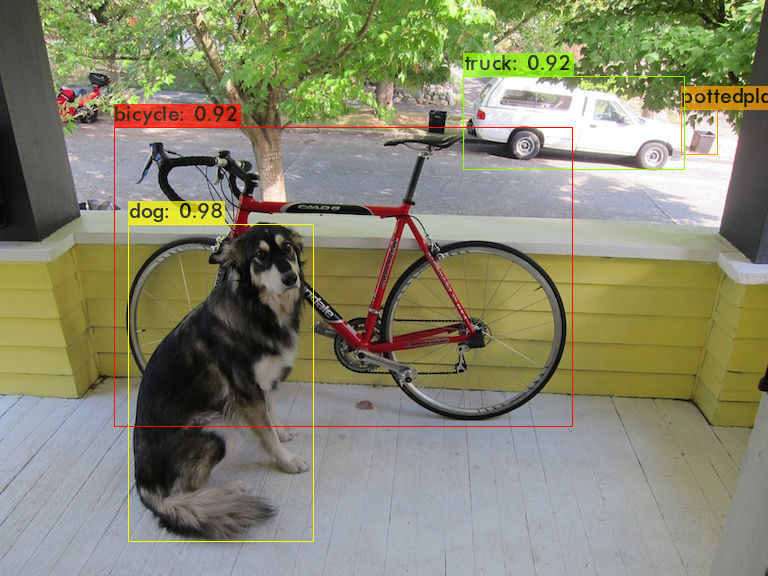
\includegraphics[width=\textwidth]{img/chapters/desarrollo/predictions.jpg}
    \caption{}
    \label{fig:predictions-darknet}
  \end{subfigure}
  \qquad\qquad
  \begin{subfigure}[b]{0.4\textwidth}
    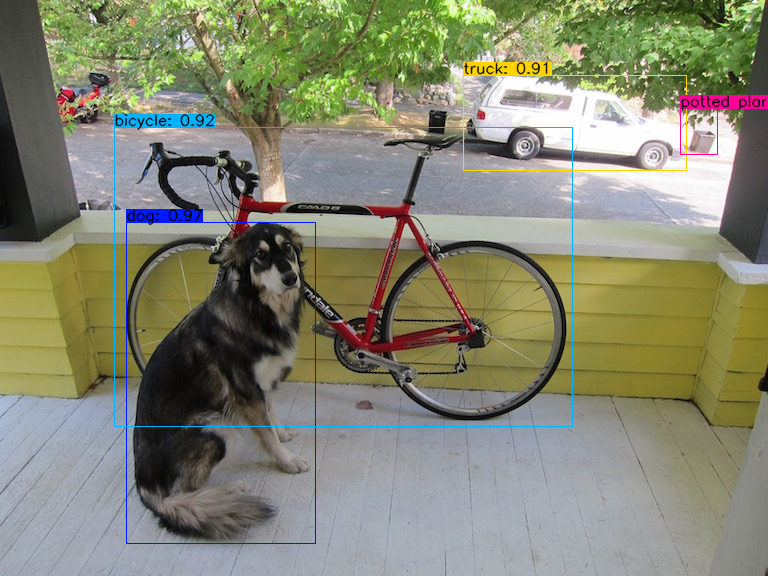
\includegraphics[width=\textwidth]{img/chapters/desarrollo/detection1.png}
    \caption{}
    \label{fig:predictions-tf}
  \end{subfigure}
  \caption{Detecciones de YOLOv4 con Darknet y Tensorflow.
    (\protect\subref{fig:predictions-darknet}) Detección de YOLOv4 con Darknet.
    (\protect\subref{fig:predictions-tf}) Detección de YOLOv4 con Tensorflow.}
  \label{fig:predictions-darknet-tf}
\end{figure}

\textcolor{red}{Dado que el algoritmo de seguimiento es una extensión del algoritmo de detección se comentará solamente el de DeepSORT para no comentar dos veces los mismos fragmentos del código, haciendo referencia al código del apéndice en las funciones más relevante del script de detección y seguimiento}.

\newpage

\section{Datasets utilizados para el entrenamiento de YOLOv4}
\label{sec:datasets-utilizados}

\textcolor{red}{Hacer introducción y ajustar imágenes de esta sección antes de seguir con la siguiente}

asdfasdf

asdfasdf

asdfasdf

asdfasdf

asdfasdf

asdfasdf

asdfasdf

asdfasdf

\subsection{MS COCO Dataset}
\label{subsec:coco-dataset}

El dataset \gls{coco} \cite{lin2015microsoft} es un conjunto de datos de referencia utilizado para evaluar el rendimiento de los modelos entrenados por visión por computadora. Está diseñado para representar una amplia gama de objetos que encontramos regularmente en la vida cotidiana.

\begin{figure}[ht]
\centering
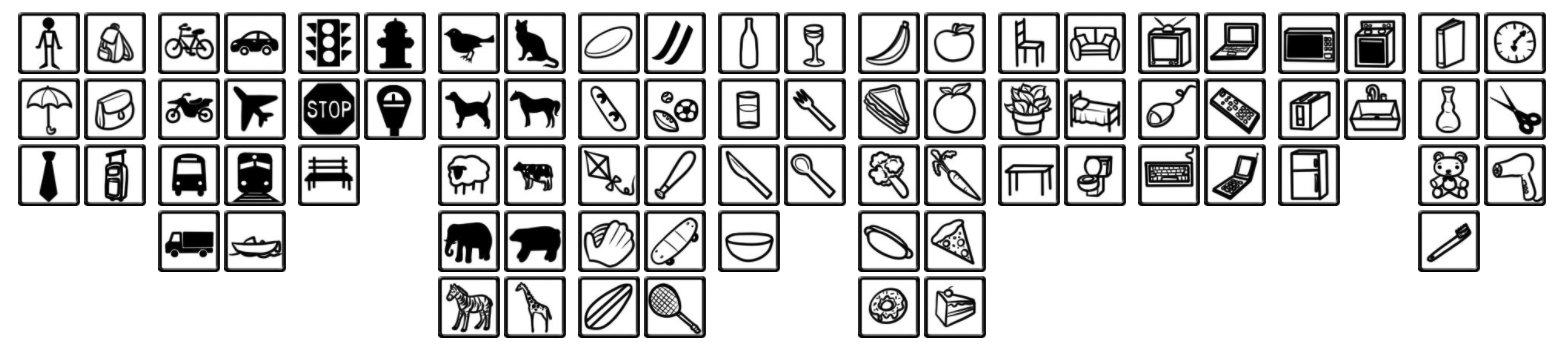
\includegraphics[width=0.9\textwidth]{img/chapters/desarrollo/cocodataset.png}
\caption{\label{fig:cocodataset}Categorías de objetos del dataset MS COCO \cite{coco-official-website}}
\end{figure}

\gls{coco} está etiquetado en un formato especial llamado COCO JSON, y proporciona datos para entrenar modelos supervisados de visión por computadora que son capaces de identificar los objetos comunes del conjunto de datos. Estos modelos están lejos de ser perfectos, por lo que el dataset \gls{coco} proporciona un punto de referencia para evaluar la mejora periódica de estos modelos a través de la investigación en visión por computadora.

Otra motivación para el dataset \gls{coco} es proporcionar un conjunto de datos base para entrenar modelos de visión por computadora. Una vez entrenado el modelo, se puede perfeccionar para aprender otras tareas, como datasets personalizados.

\subsubsection*{Tareas de MS COCO}
\label{subsubsec:tareas-coco}

\gls{coco} tiene múltiples tareas de visión por computadora. A continuación, se enumeran en orden decreciente en base a su uso:

\begin{itemize}
    \item \textbf{Detección de objetos}: los objetos se anotan con un cuadro delimitador y una etiqueta de clase. El dataset \gls{coco} tiene 121.408 imágenes para detección de objetos, 883.331 anotaciones de objetos, 80 clases (ver figura \ref{fig:cocodataset}) y una resolución media de imagen de 640x480.
    
    \begin{figure}[ht]
    \centering
    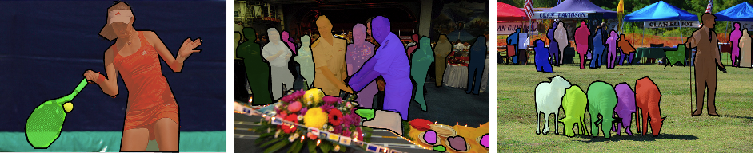
\includegraphics[width=0.65\textwidth]{img/chapters/desarrollo/detection-splash.png}
    \caption{\label{fig:detection-splash}MS COCO detección de objetos \cite{coco-official-website}}
    \end{figure}
    
    \item \textbf{Segmentación semántica}: los límites de los objetos se etiquetan con una máscara y las clases de objetos se etiquetan con una etiqueta de clase. La segmentación semántica requiere modelos para trazar los límites entre los objetos.
    
    \begin{figure}[ht]
    \centering
    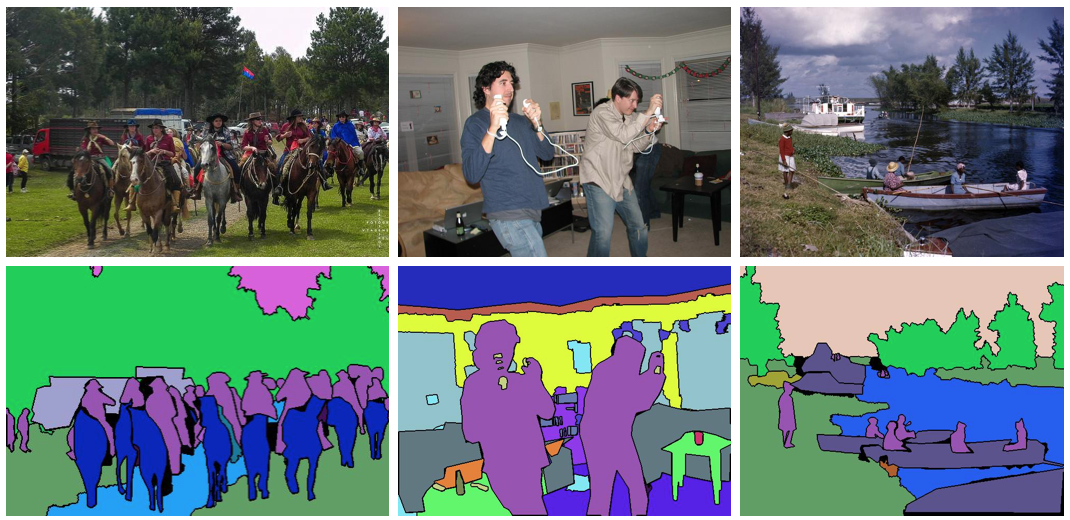
\includegraphics[width=0.6\textwidth]{img/chapters/desarrollo/panoptic-splash.png}
    \caption{\label{fig:panoptic-splash}MS COCO segmentación semántica \cite{coco-official-website}}
    \end{figure}    
    
    \item \textbf{Detección de puntos clave}: las personas son etiquetadas con puntos claves de interés (como pueden ser codos, rodillas o cabezas). El dataset \gls{coco} dispone de 250.000 personas con puntos clave etiquetados.
    
    \begin{figure}[ht]
    \centering
    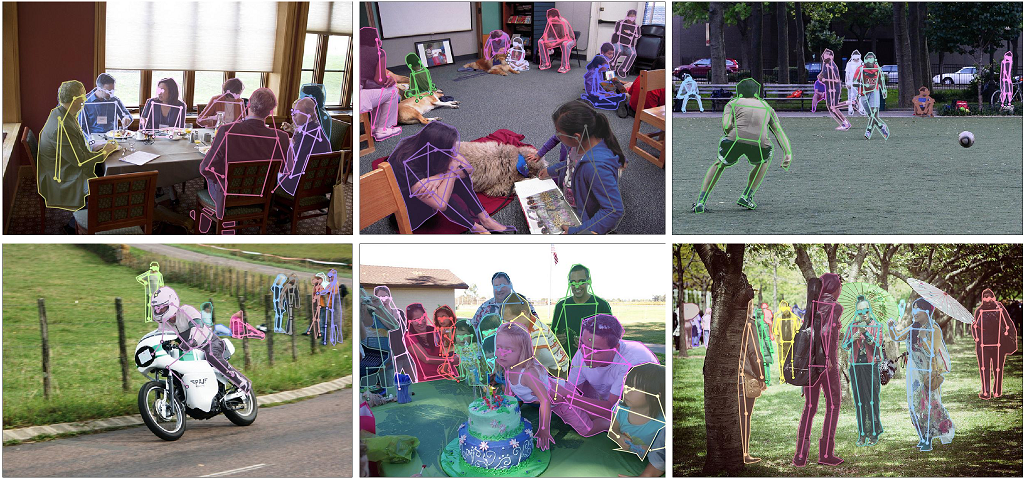
\includegraphics[width=0.6\textwidth]{img/chapters/desarrollo/keypoints-splash-big.png}
    \caption{\label{fig:keypoints-splash-big}MS COCO detección de puntos clave \cite{coco-official-website}}
    \end{figure}    
    
\end{itemize}

\subsection{Open Images Dataset v4}
\label{subsec:OIDv4-dataset}

\gls{oidv4} \cite{Kuznetsova_2020} es un conjunto de datos de 9,2 millones de imágenes con anotaciones en formato .txt unificadas para la clasificación de imágenes, detección de objetos y detección de relaciones visuales (ver figura \ref{fig:example-annotations-oidv4}). Las imágenes tienen una licencia Creative Commons Attribution que permite compartir y adaptar el material descargado de Flickr sin una lista predefinida de nombres de clases o etiquetas.

\begin{figure}[ht]
\centering
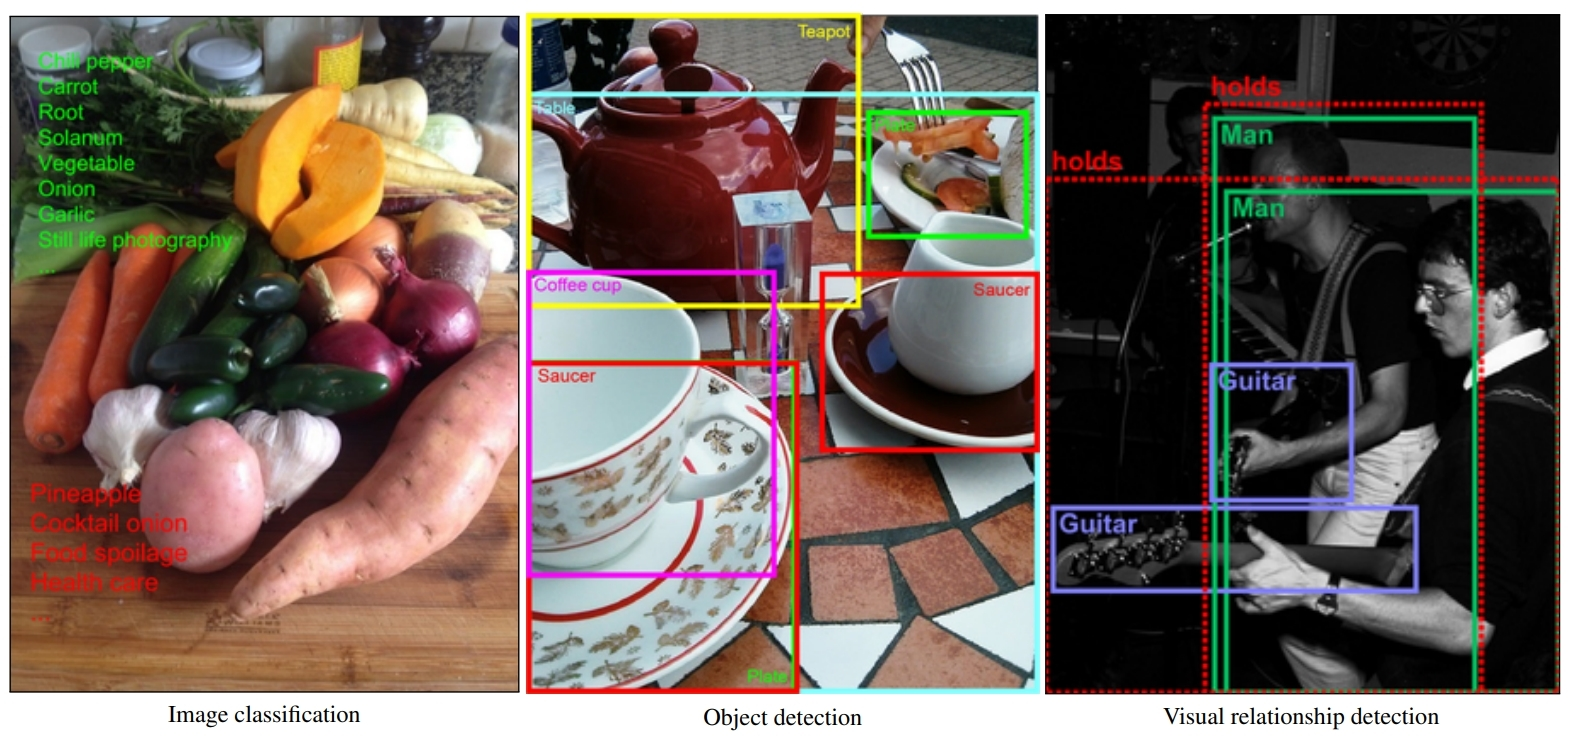
\includegraphics[width=0.6\textwidth]{img/chapters/desarrollo/example-annotations-oidv4.jpg}
\caption{\label{fig:example-annotations-oidv4}Ejemplo anotaciones en Open Images Dataset v4 \cite{Kuznetsova_2020}}
\end{figure}

\gls{oidv4} ofrece una gran escala en varias dimensiones: 30,1 millones de etiquetas a nivel de imagen para 19,8 mil conceptos, 15,4 millones de cuadros delimitadores para las 600 clases de objetos que se muestran en la figura \ref{fig:oidv4dataset}, y 375 mil anotaciones de relaciones visuales que involucra 57 clases. Para la detección de objetos se proporciona más de 15 veces cuadros delimitadores que otros grandes datasets como \gls{coco} o ImageNet. Las imágenes suelen mostrar escenas complejas con varios objetos (de promedio tiene 8 objetos anotados por imagen). 

\begin{figure}[ht]
\centering
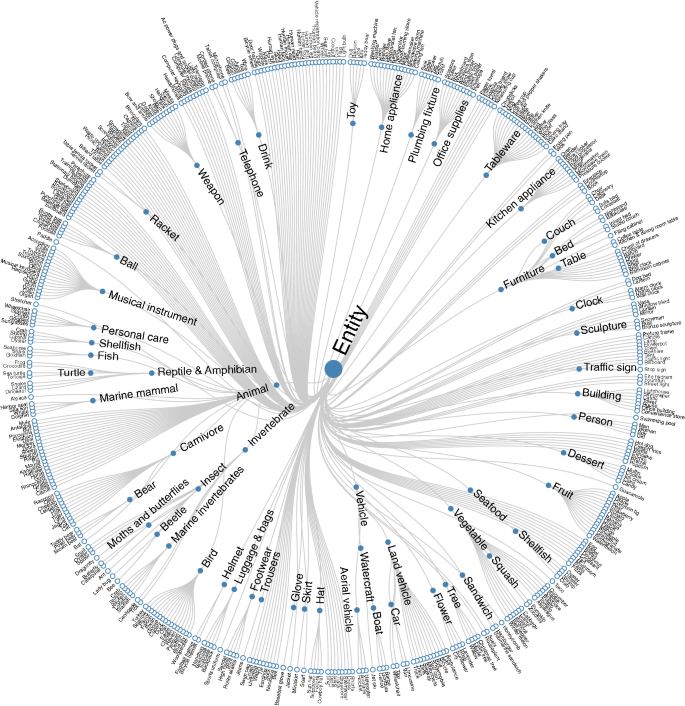
\includegraphics[width=0.65\textwidth]{img/chapters/desarrollo/oidv4-classes.png}
\caption{\label{fig:oidv4dataset}Categorías de objetos del dataset Open Images Dataset v4 \cite{Kuznetsova_2020}}
\end{figure}

\newpage

\section{Entrenamiento YOLOv4 con Open Image Dataset v4}
\label{sec:train-openimagesv4}

\textcolor{red}{Aquí explicar como he entrenado una red neuronal con otro dataset a partir del repositorio \cite{OIDv4_ToolKit}}

\textcolor{red}{Explicar que se ha tomado 1.500 imágenes de entrenamiento de las clases: person, handbag, backpack, suitcase y 300 imágenes de validación.}

\vspace{0.5cm}
\begin{lstlisting}[language=iPython,caption=Descarga dataset Open Images Dataset v4,captionpos=b,label={lst:download-oidv4}]
# Clonar el repositorio de Github
git clone https://github.com/theAIGuysCode/OIDv4_ToolKit.git
cd OIDv4_ToolKit

# Instalacion de las librerias y dependendencias
pip install -r requirements.txt

# Descarga de las imagenes de entrenamiento con un limite de 1500
python main.py downloader --classes Person Handbag Backpack Suitcase --type_csv train --limit 1500 --multiclasses 1

# Descarga de las imagenes de validacion con un limite de 300
python main.py downloader --classes Person Handbag Backpack Suitcase --type_csv validation --limit 300 --multiclasses 1

# Convertir etiquetas al formato de Darknet
python convert_annotations.py
\end{lstlisting}

\begin{figure}[ht]
\centering
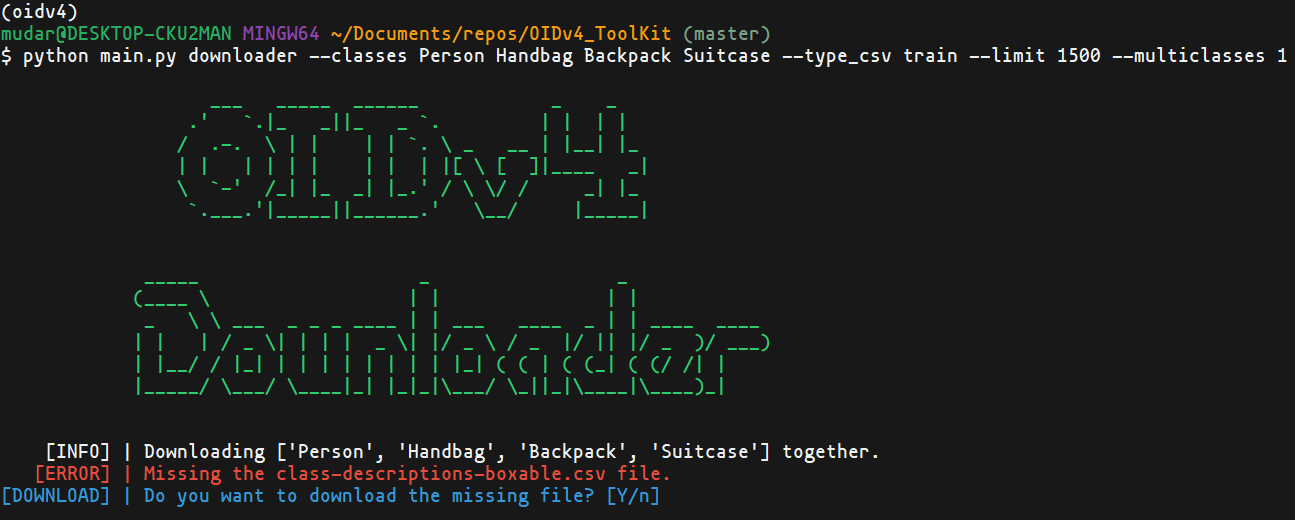
\includegraphics[width=0.55\textwidth]{img/chapters/resultados/datasets/download-oidv4.png}
\caption{\label{fig:download-oidv4}Descarga del dataset Open Images Dataset v4}
\end{figure}

\begin{figure}[ht]
\centering
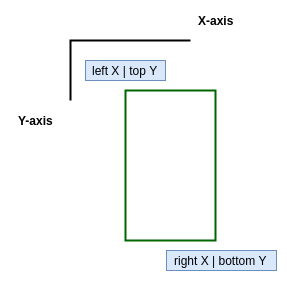
\includegraphics[width=0.45\textwidth]{img/chapters/resultados/datasets/bbox-oidv4.png}
\caption{\label{fig:bbox-oidv4}Estructura de las etiquetas de Open Images Dataset v4 \cite{OIDv4_ToolKit}}
\end{figure}

La estructura que siguen las etiquetas del dataset de Open Images Dataset v4 es la siguiente:

nombre de la clase x left top y x right bottom y

\newpage

\section{Seguimiento de personas y objetos con YOLOv4 y Deep SORT}
\label{sec:desarrollo-yolov4+deepsort}

\textcolor{red}{Aquí hacer una breve descripción de deepsort, muy breve porque ya se ha explicado en el capitulo del estado del arte, y poner imagenes de su funcionamiento sobre yolov4 en el framework tensorflow}.

\textcolor{red}{Dado que el código que se va a comentar en esta sección es bastante largo para reflejarlo se ha optado por crear un apéndice al final del documento dedicado al mismo}.

\newpage

\section{Algoritmo de detección de objetos abandonados}
\label{sec:algoritmo-object-detection}

\textcolor{red}{Dibujar el esquema que voy a seguir para determinar cuando un objeto ha sido abandonado.}
\url{https://app.diagrams.net/}

\textcolor{red}{Intentar meter toda la chicha posible. Que quede pendiente meter aquí código de lo que he implementado para que no quede todo en el aire y se vean de repente los resultados, por lo menos que se vea la función que hace la asociación de persona objeto y la función que establece si la persona ha abandonado un objeto o si el objeto esta abandonado y sin propietario.}

\textcolor{red}{Poner figura ejemplo de la hipotesis donde se hace asociacion de persona y objeto cuando se activa la alarma y cuando se determina que un objeto ha sido abandonado, en el momento de la alarma se ejecuta una cuenta atrás de 30 segundos antes de determinar que el objeto ha sido abandonado.}

\textcolor{red}{Explicar la hipótesis de cuando un objeto no tiene propietario porque se encuentra alejado de cualquier persona en los primeros fotogramas del vídeo. En este caso al pasar 15 segundos se determina que el objeto ha sido abandonado.}

Cuando se calcula se calcula la distancia entre personas y objetos de interés se calcula la media de las distancias obtenidas fotograma a fotograma en los primeros 5 segundos de vídeo. Se crea una asociación de una persona al objeto que se haya obtenido la menor distancia en el momento de la asociación, siempre y cuando esa distancia sea inferior a dos veces el ancho del cuadro limitador del objeto, para así no depender de la profundidad a la que se pueda encontrar las personas y objetos dentro del plano de visión.

\begin{figure}[ht]
\centering
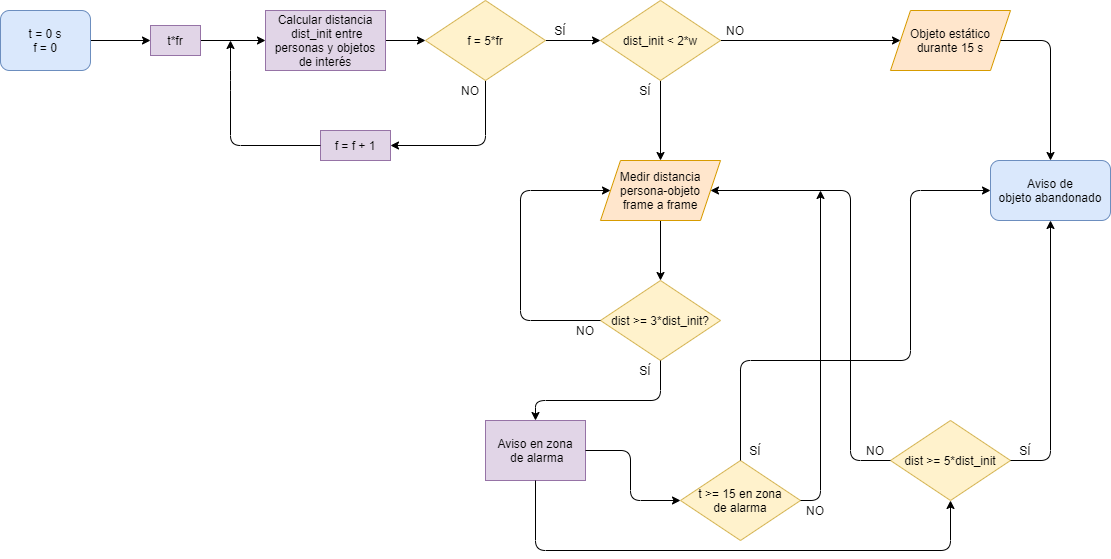
\includegraphics[width=1\textwidth]{img/chapters/desarrollo/abandoned-object-scheme.png}
\caption{\label{fig:abandoned-object-scheme}Esquema hipótesis detección objeto abandonado}
\end{figure}

\newpage

\begin{figure}[ht]
\centering
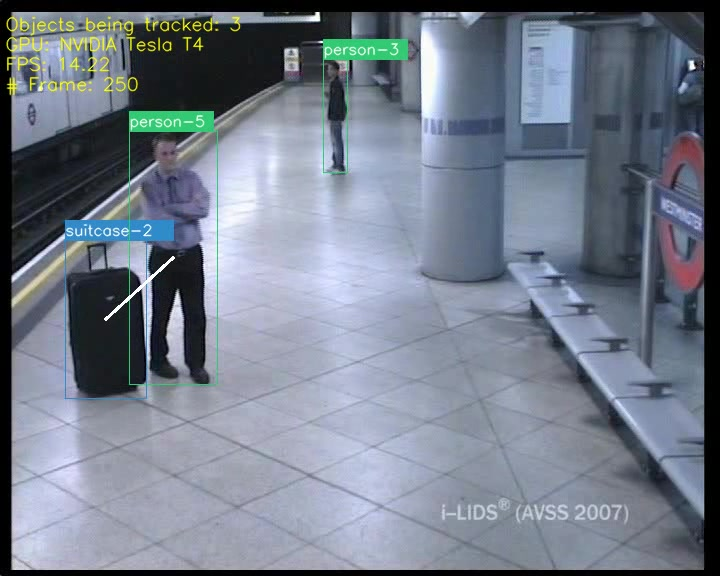
\includegraphics[width=0.4\textwidth]{img/chapters/desarrollo/link-persona-objeto.jpg}
\caption{\label{fig:link-persona-objeto}Asociación persona-objeto}
\end{figure}

Hola hola

\begin{figure}[ht]
\centering
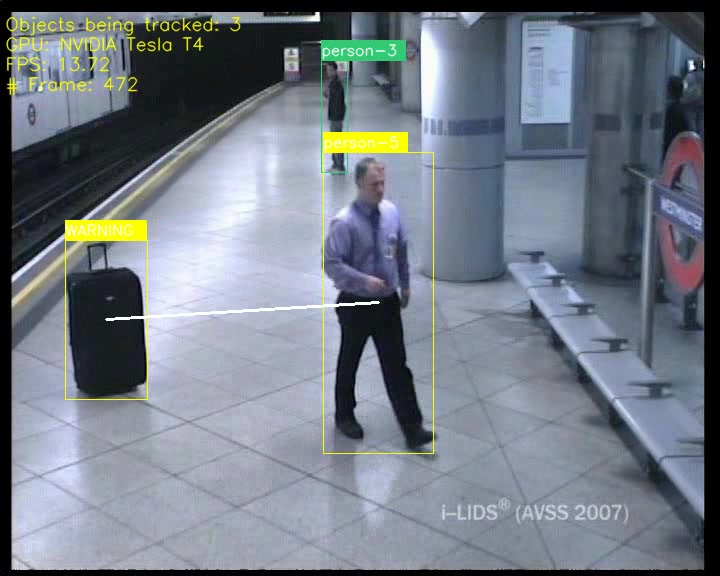
\includegraphics[width=0.4\textwidth]{img/chapters/desarrollo/warning-abandono.jpg}
\caption{\label{fig:warning-abandono}Aviso de alerta posible objeto abandonado}
\end{figure}

Hola hola

\begin{figure}[ht]
\centering
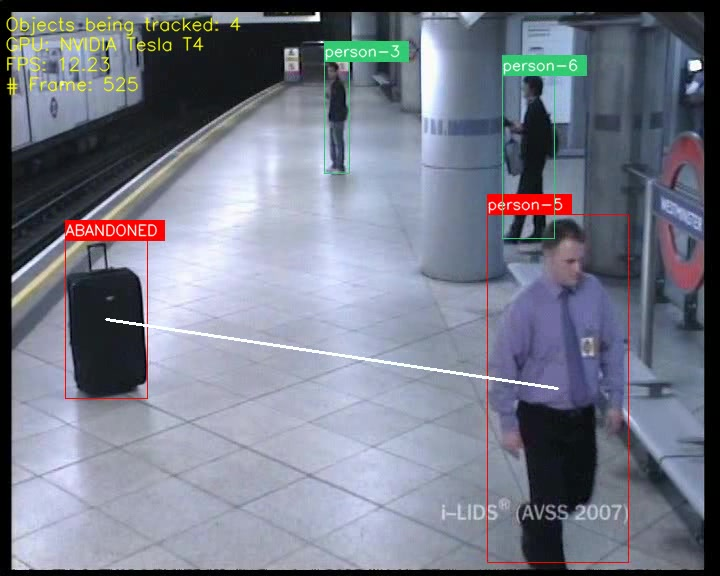
\includegraphics[width=0.4\textwidth]{img/chapters/desarrollo/abandono-objeto-avss.jpg}
\caption{\label{fig:abandono-objeto-avss}Detección de objeto abandonado}
\end{figure}

Hola hola

\newpage

\section{Conclusiones}
\label{sec:conclu-desarrollo}

\textcolor{red}{Hacer unas breves conclusiones de lo que se ha conseguido en base a los objetivos que se han marcado en la introducción de este capítulo \ldots}

\begin{algorithm}[H]
 \caption{How to write algorithms}
 \label{alg:howto}
 \KwData{this text}
 \KwResult{how to write algorithm with \LaTeX}
 initialization\;
 \While{not at end of this document}{
  read current\;
  \eIf{understand}{
   go to next section\;
   current section becomes this one\;
   }{
   go back to the beginning of current section\;
  }
 }
\end{algorithm}